\documentclass{article}
\usepackage{graphicx}
\usepackage{natbib}
\bibliographystyle{unsrt}
\usepackage{algorithm}
\usepackage{algpseudocode}

\begin{document}
\title{Big Graph Tools}
\author{Tian Yong}
\maketitle
\section{Introduction}
Many practical computing problems concern large graphs.
Standard examples include the Web graph and various social networks.
The scale of these graphs (in some cases billions of vertices,
trillions of edges) poses challenges to their efficient processing.

There are several choices to implement an algorithm to process a large graph:
\begin{itemize}
  \item Crafting a custom distributed infrastructure. This choice leaves machine learning experts repeatedly design a system and implement it.
  \item Relying on an existing distributed computing platform like MapReduce, which is not suit for graph processing.
  \item Using a single-computer graph algorithm library limiting the scale of problems that can addressed.
  \item Using an parallel graph system, fault tolerance or not.
\end{itemize}

This paper will introduce four representative big graph processing tools, which are
Pregel\cite{malewicz2010pregel}, GraphLab\cite{low2010graphlab}, PowerGraph\cite{gonzalez2012powergraph}
and GraphChi~\cite{kyrola2012graphchi}. Before going into the details, it's better
to introduce the common \textbf{data graph model}.
The data graph $G = (V, E)$ encodes both the problem specific sparse computational
structure and directly modifiable program state.
The user can associate arbitrary blocks of data (or parameters) with each
vertex and directed edge in $G$. We denote the data associated with vertex $v$ by $D_v$ ,
and the data associated with edge $(u,v)$ by $D_{(u,v)}$.
Although the methodology of each tool differs from each other, they do share
the same data model with slight difference.

\section{Pregel}
Pregel is a bulk synchronous message passing abstraction in
which all vertex-programs run simultaneously in a sequence of super-steps.
The input to a Pregel computation is a directed graph in
which each vertex is uniquely identified by a string vertex
identifier. Each vertex is associated with a modifiable, user
defined value. The directed edges are associated with their
source vertices, and each edge consists of a modifiable, user
defined value and a target vertex identifier.

\subsection{Computation Model}
Pregel computations consist of a sequence of iterations, called \emph{supersteps}. During a superstep the framework invokes a user-defined function for each vertex, conceptually in parallel.
The function specifies behavior at a single vertex $V$ and a
single superstep $S$. It can read messages sent to $V$ in superstep $S-1$, send messages to other vertices that will be received at superstep $S + 1$, and modify the state of $V$ and
its outgoing edges. Messages are typically sent along outgoing edges,
 but a message may be sent to any vertex whose
identifier is known.  All communication is from superstep $S$ to
superstep $S + 1$. In supersteps, vertex can even change the topology of the graph.

Algorithm termination is based on every vertex voting to
halt. In superstep 0, every vertex is in the active state; all
active vertices participate in the computation of any given
superstep. A vertex deactivates itself by voting to halt. This
means that the vertex has no further work to do unless triggered externally,
and the Pregel framework will not execute
that vertex in subsequent supersteps unless it receives a message.
If reactivated by a message, a vertex must explicitly deactivate itself again.
The algorithm as a whole terminates when all vertices are simultaneously
inactive and there are no messages in transit. This state transition
model is illustrated in figure \ref{SMachine}.


\begin{figure}
  \centering
  % Requires \usepackage{graphicx}
  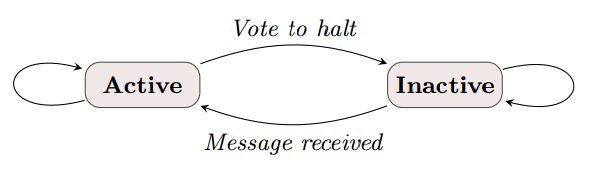
\includegraphics[width=\textwidth]{pregel_vertext_machine.PNG}\\
  \caption{Pregel Vertext State Machine}\label{SMachine}
\end{figure}

Figure \ref{pregel_max} illustrates these concepts using a simple example:
given a strongly connected graph where each vertex contains
a value, it propagates the largest value to every vertex. In
each superstep, any vertex that has learned a larger value
from its messages sends it to all its neighbors. When no
further vertices change in a superstep, the algorithm terminates.
\begin{figure}
  \centering
  % Requires \usepackage{graphicx}
  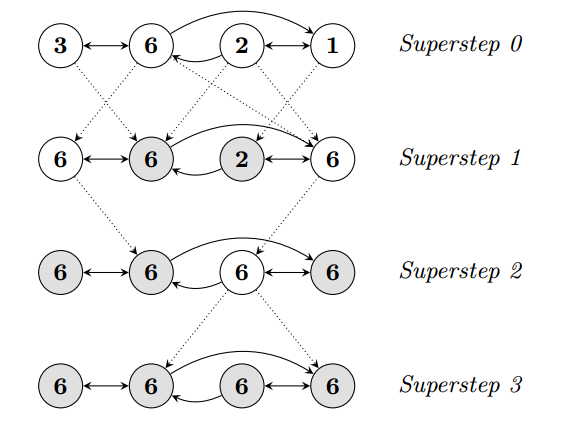
\includegraphics[width=\textwidth]{pregel_max_example.PNG}\\
  \caption{Maximum Value Example. Dotted lines
  are messages. Shaded vertices have voted to halt.}\label{pregel_max}
\end{figure}

\subsection{Pregel API}
Writing a Pregel program involves subclassing the predefined $Vertex$ class.
Users have to overrides several method to address their need.
The \textbf{Compute()} will be executed at each active vertex in every superstep.
Predefined Vertex methods allow Compute() to query information about the current
vertex and its edges, and to send messages to other vertices. Compute() can inspect the value
associated with its vertex via \textbf{GetValue()} or modify it via
\textbf{MutableValue()}. It can inspect and modify the values of
out-edges using methods supplied by the out-edge iterator.
These state updates are visible immediately. Since their visibility is confined to
the modified vertex, there are no data races on concurrent value access from different vertices.
Pregel introduces commutative associative message
\textbf{combiners} which are user defined functions that merge
messages destined to the same vertex.

The values associated with the vertex and its edges are the
only per-vertex state that persists across supersteps.
Limiting the graph state managed by the framework to a single
value per vertex or edge simplifies the main computation
cycle, graph distribution, and failure recovery.

\subsection{Discussion}
Pregel is a model suitable for large-scale graph computing with production
quality, scalable, fault-tolerant implementation.
The performance, scalability, and fault-tolerance of Pregel
are already satisfactory for graphs with billions of vertices.
Assigning vertices to machines to minimize inter-machine
communication is a challenge. However, partitioning of the input
graph based on topology may suffice if the topology corresponds to the message traffic, but it may not.
Pregel is designed for sparse graphs where communication occurs mainly over edges, and we do not expect that
focus to change. Although care has been taken to support
high fan-out and fan-in traffic, performance will suffer when
most vertices continuously send messages to most other vertices.

\section{GraphLab}
GraphLab is an asynchronous distributed shared memory abstraction in which vertex-programs have shared
access to a distributed graph with data stored on every vertex and edge.
GraphLab exploits the sparse structure and common computational patterns of ML algorithms. it
enables ML experts to easily design and implement efficient scalable parallel algorithms by composing problem
specific computation, data-dependencies, and scheduling.

\subsection{Data Model}
The GraphLab data model consists of two parts: a directed \emph{data graph} and a \emph{shared data table}. The data graph is arbitrary data block associated
with vertex or edges in a graph while a shared data table(SDT) is an associative map between keys and arbitrary blocks of data to support globally shared state or data.

\subsection{User Defined Computation}
There are two kinds of computation in GraphLab: update and sync. Update functions are permitted to access and modify overlapping contexts in the graph and do local computations. Sync is used to global aggregation and it runs concurrently with update functions.


A GraphLab update function is a stateless user-defined
function which operates on the data associated with small
neighborhoods in the graph and represents the core element
of computation. Given arbitrary vertex $v$, $S_v$ represents the
neighborhood of $v$ which consists of $v$, its adjacent edges
(both inbound and outbound) and its neighboring vertices.
And $D_{S_v}$ stands for the data corresponding to the neighborhood $S_v$
. In addition to $D_{S_v}$, update functions also have read-only access, to the shared
data table $T$. An update function $f$ to the vertex $v$ is:
\begin{equation}
  D_{S_v} \leftarrow f(D_{S_v}, T).
\end{equation}

A GraphLab program may consist of
multiple update functions and it is up to the scheduling
model to determine which update functions
are applied to which vertices and in which parallel order.


The sync mechanism aggregates data across all vertices in
the graph and its result is associated with a particular entry int the SDT. To invoke a sync mechanism, user
should provide a key $k$, a \textbf{fold function}(Eq. (\ref{fold_function})), an \textbf{appply function}(Eq. (\ref{apply_function})) as well as an initial value $r^{(0)}_k$ to the SDT.
\begin{equation}\label{fold_function}
r^{i+1}_k \leftarrow Fold_k (D_v, r^{i}_k)
\end{equation}
\begin{equation}\label{apply_function}
  T[k] \leftarrow Apply_k(r_k^{(|V|)})
\end{equation}

When the sync mechanism is invoked, the algorithm in
Alg.\ref{sync_algo} uses the $Fold_k $
function to sequentially aggregate
data across all vertices. The sync mechanism can be set to run periodically in the
background while the GraphLab engine is actively applying update functions or on demand triggered by update
functions or user code. If the sync mechanism is executed
in the background, the resulting aggregated value may not
be globally consistent. Nonetheless, many ML applications
are robust to approximate global statistics.


\begin{algorithm}
\caption{Sync algorithm on k}
\label{sync_algo}
\begin{algorithmic}[1]
\Procedure {SYNC}{$k$, $r_k^{(0)}$}
    \State $t \leftarrow r_k^{(0)}$
    \ForAll {$v \in V$}
        \State $t \leftarrow Fold_k(D_v, t)$
    \EndFor
    \State $T[k] \leftarrow Apply_k(t)$

\EndProcedure


\end{algorithmic}
\end{algorithm}

\subsection{Data Consistency}
Since scopes may overlap, the simultaneous execution of
two update functions can lead to race-conditions resulting
in data inconsistency and even corruption. GraphLab provides
 a choice of three data consistency models which enable the user
  to balance performance and data consistency. The 3 models is illustrated in Figure \ref{graphlab_scope}
   by drawing their exclusion sets as a ring where no two update functions
    may be executed simultaneously if their exclusions sets overlap
\begin{figure}
  \centering
  % Requires \usepackage{graphicx}
  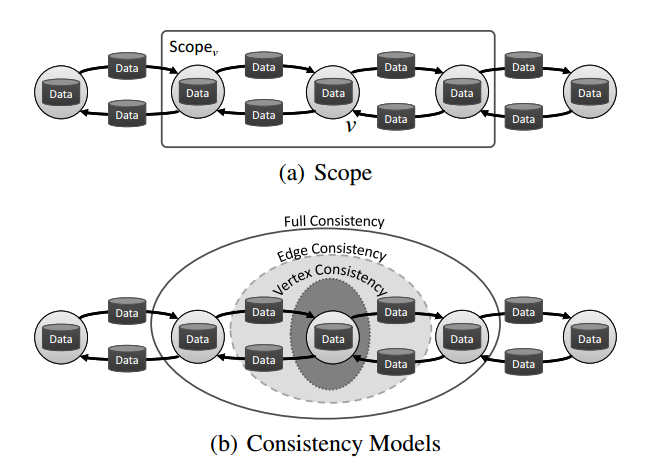
\includegraphics[width=\textwidth]{graphlab_scope}\\
  \caption{(a) The scope, $S_v$ of vertex $v$. (b). Three data consistency
   models.}\label{graphlab_scope}
\end{figure}



\subsection{Scheduling}
The GraphLab update schedule describes the order in
which update functions are applied to vertices and is represented by a parallel data-structure called the scheduler.
The scheduler abstractly represents a dynamic list of tasks
(vertex-function pairs) which are to be executed by the
GraphLab engine. GraphLab framework provides a collection of base schedules to achieve different goals.

GraphLab also provide two termination assessment methods. The first method relies on
the scheduler which signals termination when there are no
remaining tasks. The second termination
method relies on user provided termination functions which
examine the SDT and signal when the algorithm has converged.

\subsection{Assessment}
GraphLab is a parallel abstraction which achieves
a high level of usability, expressiveness and performance.
Unlike existing parallel abstractions, GraphLab supports
the representation of structured data dependencies, iterative
computation, and flexible scheduling.
The optimized shared memory implementation gives GraphLab a
state-of-the-art performance.

\section{PowerGraph}

\subsection{Challenges of Natural Graphs}
The sparsity structure of natural graphs presents a unique
challenge to efficient distributed graph-parallel computation.
One of the hallmark properties of natural graphs is their skewed
power-law degree distribution: most vertices have relatively few
neighbors while a few have many neighbors. Under a power-law degree
distribution the probability that a vertex has degree $d$ is given
by:
\begin{equation}\label{prob_degree}
  P(d) \propto d^{-\alpha}
\end{equation}
where the exponent $\alpha$ is a positive constant that controls
the ``skewness'' of the degree distribution.


The skewed degree distribution implies that a small
fraction of the vertices are adjacent to a large fraction
of the edges. For example, one percent of the vertices
in the Twitter web-graph are adjacent to nearly half of
the edges. This concentration of edges results in a star-like motif
which presents challenges, such as work balance, communication and
storage, for existing graph-parallel abstractions, which factor
computation over vertices.


\begin{algorithm}
\caption{Vertex-Program Execution Semantics}
\label{vertex_algo}
\begin{algorithmic}[1]
\State \textbf{Input}: Center vertex $u$
\If cached accumulator $a_u$ is empty
    \For neighbor $v$ in gather \_nbrs(u)
    \State $a_u \leftarrow sum(a_u, gather(D_u, D_{(u, v)}, D_v))$
    \EndFor
\EndIf
\State $D_u \leftarrow apply(D_u, a_u)$
\For neighbor v scatter\_nbrs(u)
    \State $(D_{(u, v)}, \Delta a) \leftarrow scatter(D_u, D_{(u,v)}, D_v)$
    \If $a_v$ and $\Delta a$ are not Empty
        \State $a_v \leftarrow sum(a_v, \Delta a)$
    \Else
        \State $a_v \leftarrow$ Empty
    \EndIf
\EndFor
\end{algorithmic}
\end{algorithm}

\subsection{GAS Model}
To address the challenge of computation on power-law graphs,
PowerGraph abstraction exploits the structure of vertex-programs
and explicitly factors computation over edges instead of vertices.
As a consequence, PowerGraph exposes substantially greater parallelism,
reduces network communication and storage costs, and provides a new
highly effective approach to distributed graph placement.

\begin{figure}
  \centering
  % Requires \usepackage{graphicx}
  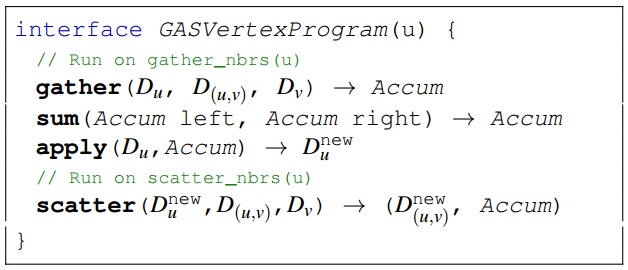
\includegraphics[width=\textwidth]{GAS.png}\\
  \caption{All PowerGraph programs must implement the stateless
  gather, sum, apply, and scatter functions.}\label{GAS_inter}
\end{figure}


Computation in the PowerGraph abstraction is encoded
as a state-less vertex-program which implements the
GASVertexProgram interface (Fig. \ref{GAS_inter}) and therefore
explicitly factors into the gather, sum, apply, and scatter functions.
Each function is invoked in stages by the PowerGraph engine following
the semantics in Alg.\ref{vertex_algo}. By factoring the vertex-program,
the PowerGraph execution engine can distribute a single vertex-program over
multiple machines and move computation to the data.


During the gather phase the gather and sum functions are used as a map and
reduce to collect information about the neighborhood of the vertex.
The gather function is invoked in parallel on the edges adjacent to $u$. The
particular set of edges is determined by $gather\_nbrs$ which can be $none$,
$in$, $out$, or $all$. The gather function is passed the data on the adjacent
vertex and edge and returns a temporary accumulator (a user defined type).
The result is combined using the commutative and associative sum operation.
The final result $a_u$ of the gather phase is passed to the $apply$ phase and
cached by PowerGraph.


After the $gather$ phase has completed, the $apply$ function takes the final
accumulator and computes a new vertex value $D_u$ which is atomically written
back to the graph. The size of the accumulator $a_u$ and complexity of the
apply function play a central role in determining the network and storage
efficiency of the PowerGraph abstraction and should be sub-linear and ideally
constant in the degree.


During the $scatter$ phase, the scatter function is invoked in parallel on
the edges adjacent to $u$ producing new edge values $D_{(u,v)}$ which are
written back to the data graph. As with the gather phase, the $scatter\_nbrs$
determines the particular set of edges on which scatter is invoked. The scatter
function returns an optional value $\Delta a$ which is used to dynamically
update the cached accumulator $a_v$ for the adjacent vertex.

\subsection{Delta Chaching}
In many cases a vertex-program will be triggered in response to a change in a
few of its neighbors. The gather operation is then repeatedly invoked on all
neighbors, many of which remain unchanged, thereby wasting computation cycles.
For many algorithms it is possible to dynamically maintain the result of the
gather phase $a_u$ and skip the gather on subsequent iterations. The PowerGraph
engine maintains a cache of the accumulator $a_u$ from the previous gather phase
for each vertex. The scatter function can optionally return an additional $\Delta
a$ which is atomically added to the cached accumulator $a_v$ of the neighboring
vertex $v$ using the sum function. If $\Delta a$ is not returned, then the
neighbor`s cached $a_v$ is cleared forcing a complete gather on the subsequent
execution of the vertex-program on the vertex $v$. When executing the vertex-program
on $v$ the PowerGraph engine uses the cached $a_v$ if available, bypassing the
gather phase.


\subsection{Initiating Future Computation}
The PowerGraph engine maintains a set of active vertices
on which to eventually execute the vertex-program. The
user initiates computation by calling $Activate(v)$ or
$Activateall()$. The PowerGraph engine then proceeds to
execute the vertex-program on the active vertices until
none remain. Once a vertex-program completes the scatter
phase it becomes inactive until it is reactivated.

Vertices can activate themselves and neighboring vertices.
Each function in a vertex-program can only activate vertices
visible in the arguments to that function.

The order in which activated vertices are executed is up
to the PowerGraph execution engine. The only guarantee
is that all activated vertices are eventually executed. This
flexibility in scheduling enables PowerGraph programs
to be executed both synchronously and asynchronously,
leading to different tradeoffs in algorithm performance,
system performance, and determinism.


\subsection{Distributed Graph Placement}

\begin{figure}
  \centering
  % Requires \usepackage{graphicx}
  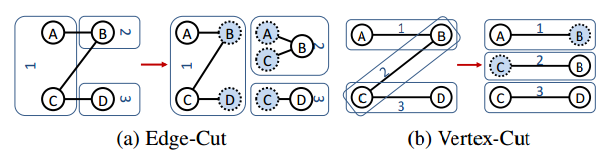
\includegraphics[width=\textwidth]{cut.png}\\
  \caption{(a)An edge-cut and(b)vertex-cut of a graph
  into   three parts. Shaded vertices are ghosts and
  mirrors respectively.}\label{cut}
\end{figure}

The placement of the data-graph structure and data plays
a central role in minimizing communication and ensuring
work balance. A common approach to placing a graph on a
cluster of $p$ machines is to construct a balanced $p$-way
edge-cut (e.g., Fig. \ref{cut}a) in which vertices are evenly
assigned to machines and the number of edges spanning machines
is minimized. Unfortunately, the tools for constructing balanced
edge-cuts perform poorly on power-law graphs. When the graph
is difficult to partition, both GraphLab and Pregel resort
to hashed (random) vertex placement. While fast and easy to
implement, hashed vertex placement cuts most of the edges. If
vertices are randomly assigned to $p$ machines then the expected
fraction of edges cut is:
\begin{equation}
  \textbf{E}[\frac{|Edges Cut|}{|E|} = 1 - \frac{1}{p}.
\end{equation}

For a power-law graph with exponent $\alpha$, the expected
number of edges cut per-vertex is:
\begin{equation}
  \textbf{E}[\frac{|Edges Cut|}{|V|}]=(1-\frac{1}{p})\textbf{E}
  [D[v]]=(1-\frac{1}{p})\frac{h_{|V|}(\alpha - 1)}{h_{|V|}}
\end{equation}

where the $h_{|V|}=\sum_{d=1}^{|V|-1}d^{-\alpha}$ is the normalizing
constant of the power-law Zipf ditribution.

Every cut edge contributes to storage and network overhead since
both machines maintain a copy of the adjacency information and
in some cases, a local copy of the vertex and edge data. For example
in Fig. \ref{cut}a we construct a three-way edge-cut of a four vertex
graph resulting in five ghost vertices and all edge data being
replicated. Any changes to vertex and edge data associated with
a cut edge must be synchronized across the network. For example,
using just two machines, a random cut will cut roughly half the edges,
requiring$|E|/2$ communication.

\subsection{Balanced $p$-way Vertex-Cut}
By factoring the vertex program along the edges in the
graph, The PowerGraph abstraction allows a single vertex-program
to span multiple machines. In Fig. \ref{vertex_cut} a single high
degree vertex program has been split across two machines
with the gather and scatter functions running in parallel
on each machine and accumulator and vertex data being
exchanged across the network.

Because the PowerGraph abstraction allows a single vertex-program
to span multiple machines, we can improve work balance and reduce
communication and storage overhead by evenly assigning edges to
machines and allowing vertices to span machines. Each machine only
stores the edge information for the edges assigned to that
machine, evenly distributing the massive amounts of edge
data. Since each edge is stored exactly once, changes to
edge data do not need to be communicated. However, changes to vertex
must be copied to all the machines it spans, thus the storage and
network overhead depend on the number of machines spanned by each vertex.
To minimize storage and network overhead, PowerGraph limit the number
of machines spanned by each vertex.


A balanced $p$-way vertex-cut formalizes this objective
by assigning each edge $e \in E$ to a machine $A(e) \in \{1,\dots,p\}$.
Each vertex then spans the set of machines $A(v) \subseteq \{1,\dots, p\}$
that contain its adjacent edges. We define the balanced vertex-cut objective:

\begin{equation}\label{replication_factor}
  \min_A \frac{1}{|V|}\sum_{v\in V}|A(v)|
\end{equation}
\begin{equation}\label{balance_cons}
  s.t. \max_m |{e \in E | A(e)=m}|, < \lambda \frac{|E|}{p}
\end{equation}


where the imbalance factor $\lambda \geq 1$ is a small constant.
The term \textbf{replicas} of a vertex $v$ denotes the $|A(v)|$
copies of the vertex $v$: each machine in $A(v)$ has a replica of $v$.
Because changes to vertex data are communicated to all replicas, the
communication overhead is also given by $|A(v)|$. The objective therefore
minimizes the average number of replicas in the graph and as a consequence
the total storage and communication requirements of the PowerGraph engine.

For each vertex $v$ with multiple replicas, one of the
replicas is randomly nominated as the \textbf{master}
which maintains the master version of the vertex data.
All remaining replicas of $v$ are then \textbf{mirrors}
and maintain a local cached read-only copy of the vertex data.
For instance, in Fig. \ref{vertex_cut}b we construct a three-way
vertex-cut of a graph yielding only 2 mirrors. Any changes
to the vertex data (e.g., the Apply function) must be made to
the master which is then immediately replicated to all mirrors.

Vertex-cuts address the major issues associated with
edge-cuts in power-law graphs. Percolation theory
suggests that power-law graphs have good vertex-cuts.
Intuitively, by cutting a small fraction of the very high
degree vertices we can quickly shatter a graph.
Furthermore, because the balance constraint (Eq.\ref{balance_cons})
ensures that edges are uniformly distributed over machines, we
naturally achieve improved work balance even in the presence of
very high-degree vertices.

The simplest method to construct a vertex cut is to
randomly assign edges to machines. Random (hashed)
edge placement is fully data-parallel, achieves nearly perfect
balance on large graphs, and can be applied in the
streaming setting. In the following theorem, we relate the
expected normalized replication factor (Eq. \ref{replication_factor})
to the number of machines and the power-law constant $\alpha$.
It can be proofed that a random vertex-cut on p machines has an expected replication:
\begin{equation}
  \textbf{E}[\frac{1}{|V|}\sum_{v\in V}|A(v)|] = \frac{p}{|V|}
  \sum_{v \in V}(1 - (1-\frac{1}{p})^{D[v]}).
\end{equation}

where $D[v]$ denotes the degree of vertex $v$. For a power law graph the
expected replication is determined entirely by the power-law constant
$\alpha$:
\begin{equation}
  \textbf{E}[\frac{1}{|V|}\sum_{v \in V}|A(v)|] =
  p - \frac{p}{h_{|V|}(\alpha)} \sum_{d=1}^{|V| - 1} (\frac{p-1}{p})^d
   d^{- \alpha},
\end{equation}

where $h_{|V|}=\sum_{d=1}^{|V|-1}d^{- \alpha}$ is the normalizing constant
of the power-law Zipf distribution.

While lower $\alpha$ values (more high-degree vertices) imply a higher
replication factor the effective gains of vertex-cuts relative to edge
cuts actually increase with lower $\alpha$.


Finally, the vertex cut model is also highly effective for
regular graphs since in the event that a good edge-cut can
be found it can be converted to a better vertex cut.
For a given an edge-cut with $g$ ghosts, any vertex cut along
the same partition boundary has strictly fewer than $g$ mirrors.

\subsection{Greedy Vertex-Cuts}
It can be improved upon the randomly constructed vertex cut by
de-randomizing the edge-placement process. The
resulting algorithm is a sequential greedy heuristic which
places the next edge on the machine that minimizes the
conditional expected replication factor. To construct the
de-randomization we consider the task of placing the $i+1$
edge after having placed the previous $i$ edges. Using the
conditional expectation we define the objective:

\begin{equation}
  \arg \min_k E[\sum_{v \in V}|A(v)| | A_i, A(e_{i+1}=k],
\end{equation}

where $A_i$ is the assignment for the previous $i$ edges.
we obtain the following edge placement rules for the edge
$(u,v)$:

\begin{itemize}
  \item If $A(u)$ and $A(v)$ intersect, then the edge should be
  assigned to a machine in the intersection.
  \item If $A(u)$ and $A(v)$ are not empty and do not intersect,
  then the edge should be assigned to one of the machines
  from the vertex with the most unassigned edges.
  \item If only one of the two vertices has been assigned, then
  choose a machine from the assigned vertex.
  \item If neither vertex has been assigned, then assign the
  edge to the least loaded machine.
\end{itemize}

Because the greedy-heuristic is a de-randomization it is
guaranteed to obtain an expected replication factor that is
no worse than random placement and in practice can be
much better. Unlike the randomized algorithm, which is
embarrassingly parallel and easily distributed, the greedy
algorithm requires coordination between machines.

\begin{figure}
  \centering
  % Requires \usepackage{graphicx}
  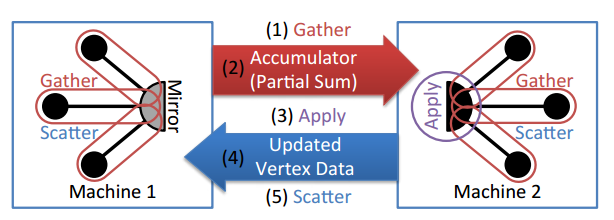
\includegraphics[width=\textwidth]{vertex_cut.png}\\
  \caption{The communication pattern of the PowerGraph abstraction when using a vertex-cut. Gather function runs locally on each machine and then one accumulators is sent from each
  mirror to the master. The master runs the apply function and
  then sends the updated vertex data to all mirrors. Finally the
  scatter phase is run in parallel on mirrors.}\label{vertex_cut}
\end{figure}



\section{Graphchi}
\subsection{Problems in Distributed Graph Systems}
Many graph systems are able to scale to graphs of
billions of edges by distributing the computation. However,
while distributed computional resources are now available
easily through the Cloud, efficient large-scale computation
on graphs still remains a challenge. To use existing graph
frameworks, one is faced with the challenge of partitioning
the graph across cluster nodes. Finding efficient graph
cuts that minimize communication between nodes, and are
also balanced, is a hard problem.
More generally, distributed systems and their users must deal with managing
a cluster, fault tolerance, and often unpredictable performance.
From the perspective of programmers, debugging
and optimizing distributed algorithms is hard.

GraphChi uses a novel method, Parallel Sliding Window(PSW) to
address this problem and achieved a amazing result: it naturally implements
the asynchronous model of computation, which has the the ability to
do advanced graph computation on just a personal computer, handling graphs
with billions of edges.

\subsection{Parallel Sliding Windows}
In many algorithms, the value of a vertex only depends
on its neighbors�� values. In many case, the computer doesn't
has enough memory to store all the vertex values. As a consequence,
the program has to frequently random access the data stored in the disk.
GraphChi use PSW to solve the random access problem.
PSW method  can process a graph with
mutable edge values efficiently from disk, with only a small
number of non-sequential disk accesses, while supporting
the asynchronous model of computation. PSW processes
graphs in three stages: it 1) loads a subgraph from disk; 2)
updates the vertices and edges; and 3) writes the updated
values to disk.

\begin{figure}
  \centering
  % Requires \usepackage{graphicx}
  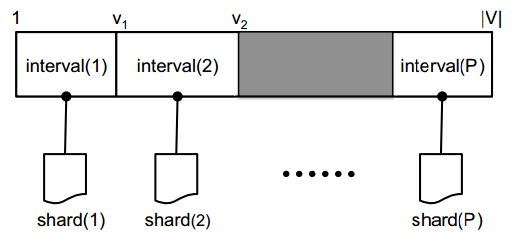
\includegraphics[width=\textwidth]{vertex_interval}\\
  \caption{The vertices of graph(V,E)are divided intoP
intervals. Each interval is associated with a shard, which
stores all edges that have destination vertex in that interval.}\label{vertex_int}
\end{figure}


Under the PSW method, the vertices $V$ of graph $G =
(V,E)$ are split into $P$ disjoint intervals. Each interval
is associated with a shard, which stores all the edges that have
destinationin the interval. Edges are stored in the order of
their source(Figure \ref{vertex_int}). Intervals are chosen to balance the
number of edges in each shard; the number of intervals,$P$,
is chosen so that any one shard can be loaded completely
into memory.

PSW does graph computation inexecution intervals,
by processing vertices one interval at a time. To create the
subgraph for the vertices in interval $p$, their edges (with
their associated values) must be loaded from disk. First,
Shard(p), which contains the in-edges for the vertices
in interval(p), is loaded fully into memory. We call thus
shard(p) the memory-shard. Second, because the edges
are ordered by their source, the out-edges for the vertices
are stored in consecutive chunks in the other shards, requiring
additional $P - 1$ block reads. Importantly, edges for
interval(p+1) are stored immediately after the edges for
interval(p). Intuitively, when PSW moves from an interval
to the next, it slides a window over each of the shards.
The other shards are called the sliding shards. Note, that if the
degree distribution of a graph is not uniform, the window
length is variable. In total, PSW requires only $P$ sequential
disk reads to process each interval. A high-level illustration
of the process is given in Figure \ref{PSW}.

\begin{figure}
  \centering
  % Requires \usepackage{graphicx}
  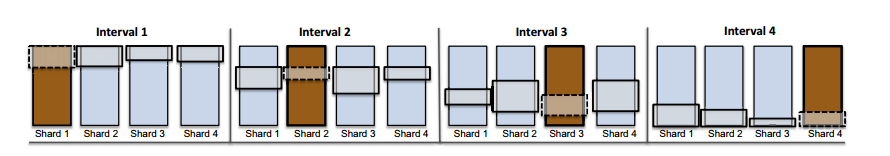
\includegraphics[width=\textwidth]{PSW.png}\\
  \caption{Visualization of the stages of one iteration of the Parallel Sliding Windows method. In this example, vertices
are divided into four intervals, each associated with a shard. The computation proceeds by constructing a subgraph of
vertices one interval a time. In-edges for the vertices are read from thememory-shard(in dark color) while out-edges
are read from each of thesliding shards. The currentsliding windowis pictured on top of each shard.}\label{PSW}
\end{figure}



After the subgraph for interval p has been fully loaded from
disk, PSW executes the user-defined update-function for
each vertex in parallel. As update-functions can modify the
edge values, to prevent adjacent vertices from accessing
edges concurrently (race conditions), we enforce external
determinism, which guarantees that each execution of PSW
produces exactly the same result. This guarantee is
straightforward to implement: vertices that have edges with both
end-points in the same interval are flagged as critical, and
are updated in sequential order. Non-critical vertices do
not share edges with other vertices in the interval, and
can be updated safely in parallel. Note, that the update of
a critical vertex will observe changes in edges done by
preceding updates, adhering to the asynchronous model of
computation. This solution, of course, limits the amount of
effective parallelism. For some algorithms, consistency is
not critical, and we allow the user to enable fully parallel updates.

Finally, the updated edge values need to be written to disk
and be visible to the next execution interval. PSW can do
this efficiently: The edges are loaded from disk in large
blocks, which are cached in memory. When the subgraph
for an interval is created, the edges are referenced as
pointers to the cached blocks; modifications to the edge values
directly modify the data blocks themselves. After finishing
the updates for the execution interval, PSW writes the
modified blocks back to disk, replacing the old data. The
memory-shard is completely rewritten, while only the active
sliding window of each sliding shard is rewritten to
disk. When PSW moves to the next interval, it reads the new
values from disk, thus implementing the asynchronous model.
The number of non-sequential disk writes for a execution interval
is $P$, exactly same as the number of reads. Note, if an
algorithm only updates edges in one direction, PSW only writes
the modified blocks to disk.

\subsection{Assessment}
Parallel Sliding Windows for the external
memory setting, exploits properties of sparse graphs
for efficient processing from disk. It requires only a small number of
sequential disk block transfers, allowing it to perform well
on both SSDs and traditional hard disks. With PSW method, GraphChi can
efficiently solve problems that were previously
only accessible to large-scale cluster computing. In addition, GraphChi relatively (per-node basis)
outperforms other existing systems, making it an attractive
choice for parallelizing multiple computations on a cluster.

\section{Conclusion}
Large-scale graph-structured computation is central to
tasks ranging from targeted advertising to natural language processing and has led to the development of
several graph-parallel abstractions including Pregel, GraphLab, PowerGraph and GraphChi.

Pregel is good at graph parallel abstraction, is easy to
reason with, and ensures deterministic computation. However it leaves
the user to architect the movement of data. Further Pregel also suffers from the curse of the slow jobs,
meaning that even a single slow job can slow down the whole
computation.

GraphLab was built with an asynchronous graph processing paradigm, which is not
affected by the curse of the slow job. It also allows dynamic iterative computations.
User-defined update functions live on each vertex and transform data in the scope of
the vertex. It can choose to trigger neighbor updates and can run without
global synchronization. Importantly, while Pregel lives with sequential
dependencies on the graphs, GraphLab allows parallelism, which is important in certain ML algorithms.

The need to reason about large-scale graph-structured data
has driven the development of new graph-parallel abstractions such as GraphLab and Pregel.
However graphs derived from real-world phenomena often exhibit power-law
degree distributions, which are difficult to partition and
can lead to work imbalance and substantially increased
communication and storage. To address these challenges, PowerGraph abstraction
exploits the Gather-Apply-Scatter model of computation to factor vertex-programs
over edges, splitting high-degree vertices and exposing
greater parallelism in natural graphs. Vertex-cuts substantially reduce the storage
and communication costs of large distributed power-law graphs.

GraphChi draw our attention from distributed solutions for graph computation with trillion edges.
With Parallel Sliding Window method, which exploits locality and properties of sparse graphs
for efficient processing from disk, GraphChi can do advanced graph computing on a personal
computer and achieve a competitive performance compared with distributed solutions
on a large cluster.
  

\bibliographystyle{unsrt}
\bibliography{ref}

\end{document}
